\documentclass[12p,a4paper]{article}
\usepackage[utf8]{inputenc}
\usepackage[T1]{fontenc,url}
\usepackage{multicol}
\usepackage{multirow}
\usepackage{parskip}
\usepackage{lmodern}
\usepackage{microtype}
\usepackage{verbatim}
\usepackage{amsmath, amssymb}
\usepackage{tikz}
\usepackage{physics}
\usepackage{mathtools}
\usepackage{algorithm}
\usepackage{algpseudocode}
\usepackage{listings}
\usepackage{enumerate}
\usepackage{graphicx}
\usepackage{float}
\usepackage{hyperref}
\usepackage{tabularx}
\usepackage{siunitx}
\usepackage{fancyvrb}
\usepackage[makeroom]{cancel}
\usepackage[margin=2.0cm]{geometry}
\renewcommand{\baselinestretch}{1}
\renewcommand{\exp}{e^}
\renewcommand{\b}{\boldsymbol}
\newcommand{\h}{\hat}
\newcommand{\m}{\mathbb}
\newcommand{\half}{\frac{1}{2}}
\renewcommand{\exp}{e^}
\renewcommand{\bar}{\overline}
\setlength\parindent{0pt}


\begin{document}
\title{MAT4110 -- Oblig 2}
\author{
    \begin{tabular}{r l}
        Jonas Gahr Sturtzel Lunde & (\texttt{jonassl})
    \end{tabular}}
% \date{}    % if commented out, the date is set to the current date

\maketitle

\hspace{10cm}

\begin{figure}[H]
    \centering
    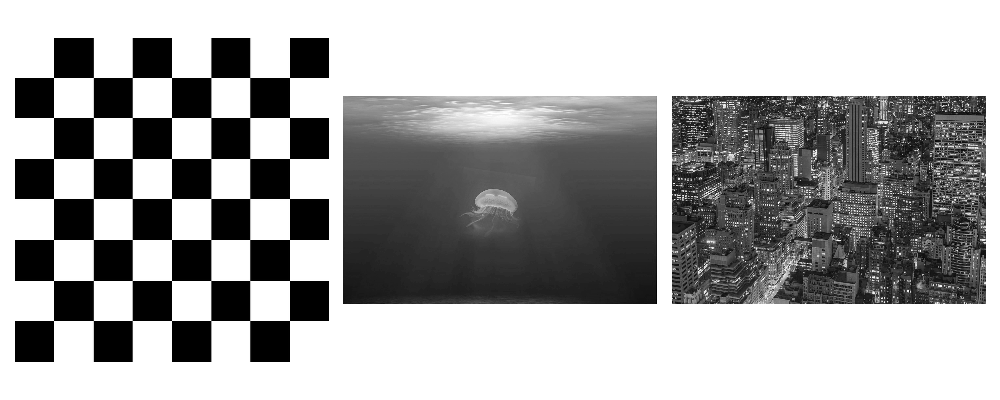
\includegraphics[width=1.0\linewidth]{../figs/original_img.png}
\end{figure}

\begin{figure}[H]
    \centering
    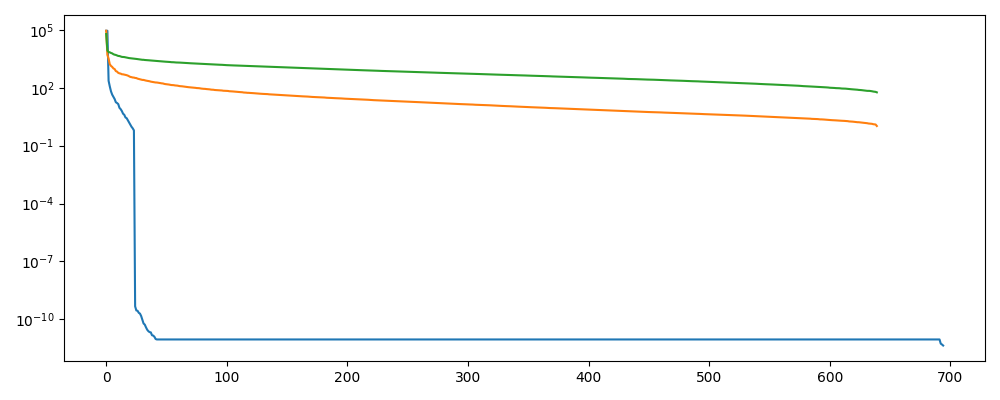
\includegraphics[width=1.0\linewidth]{../figs/singular_values.png}
\end{figure}


\begin{figure}[H]
    \centering
    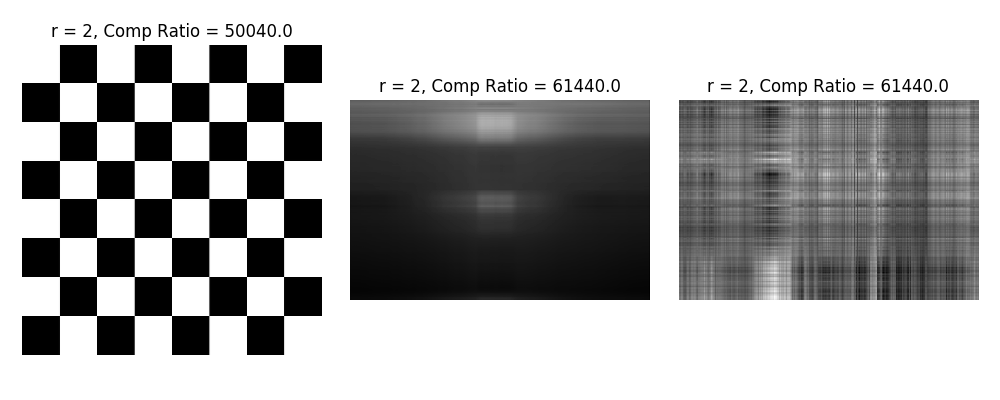
\includegraphics[width=1.0\linewidth]{../figs/img0.png}
    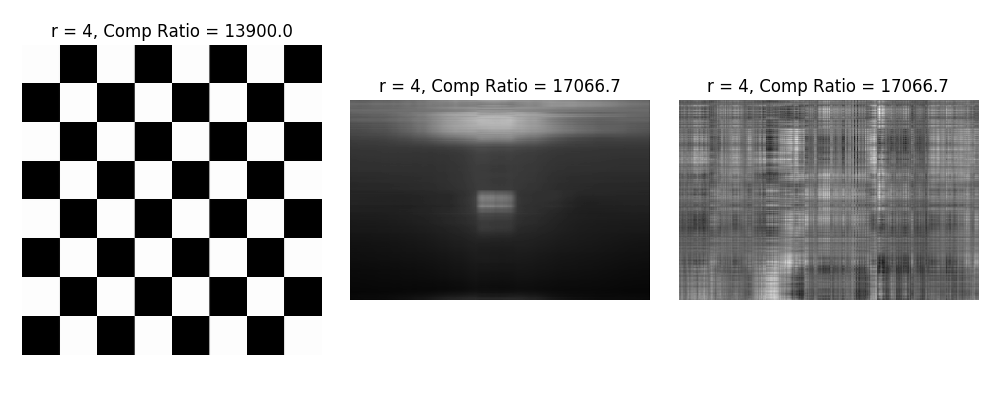
\includegraphics[width=1.0\linewidth]{../figs/img1.png}
    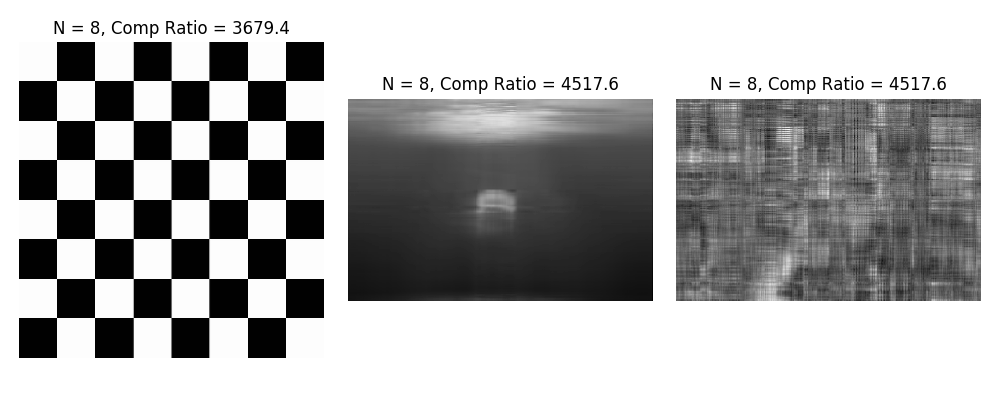
\includegraphics[width=1.0\linewidth]{../figs/img2.png}
\end{figure}

\begin{figure}[H]
    \centering
    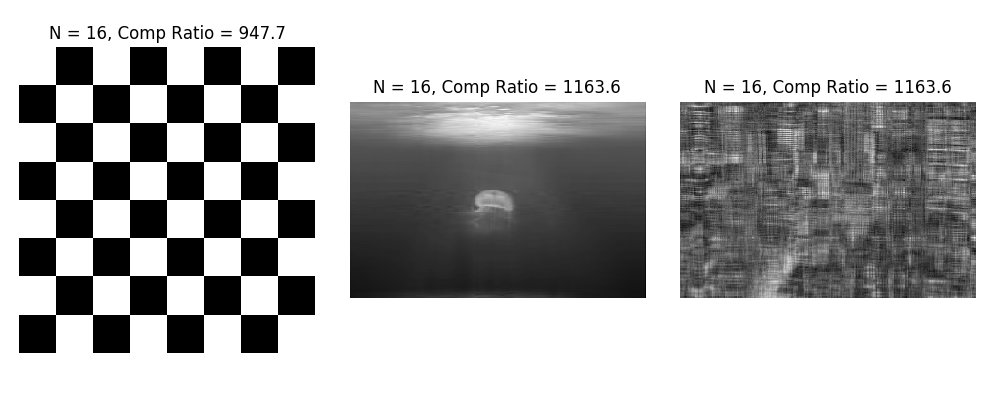
\includegraphics[width=1.0\linewidth]{../figs/img3.png}
    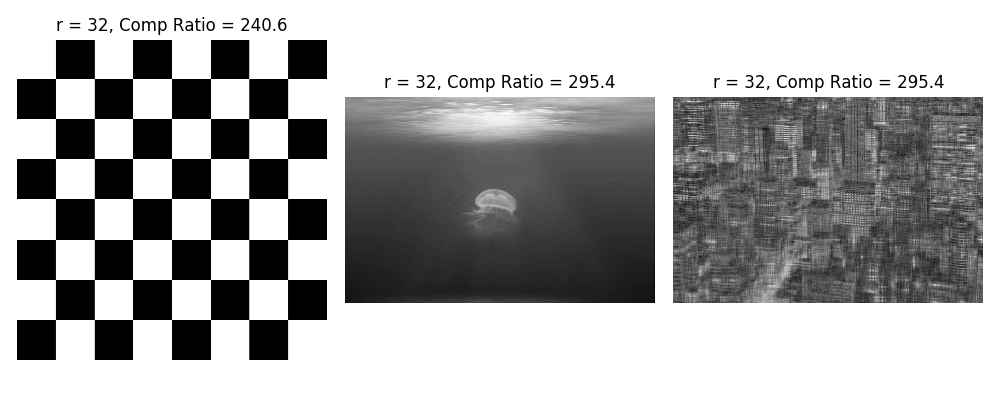
\includegraphics[width=1.0\linewidth]{../figs/img4.png}
    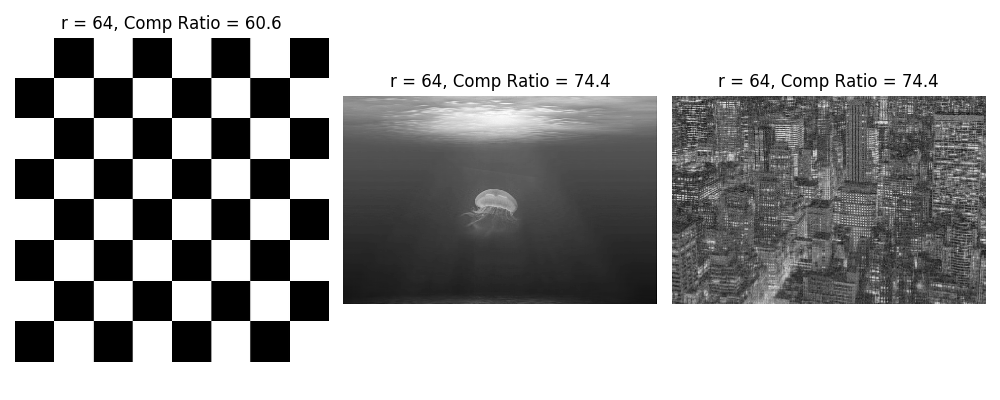
\includegraphics[width=1.0\linewidth]{../figs/img5.png}
\end{figure}

\begin{figure}[H]
    \centering
    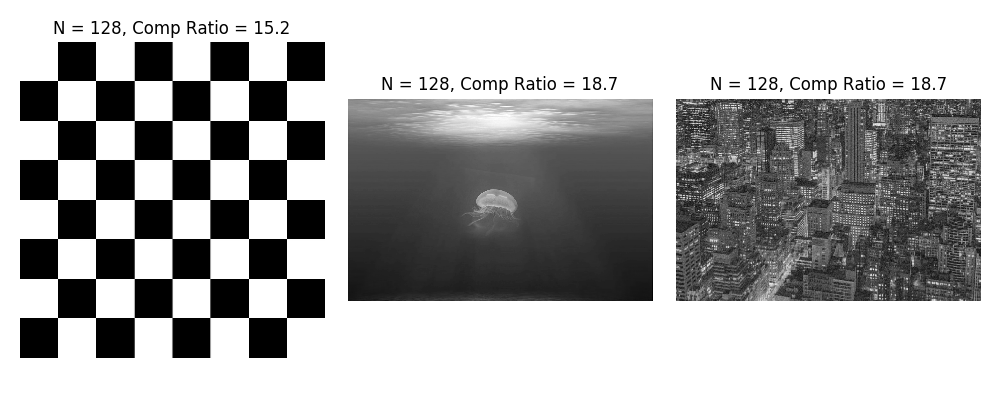
\includegraphics[width=1.0\linewidth]{../figs/img6.png}
    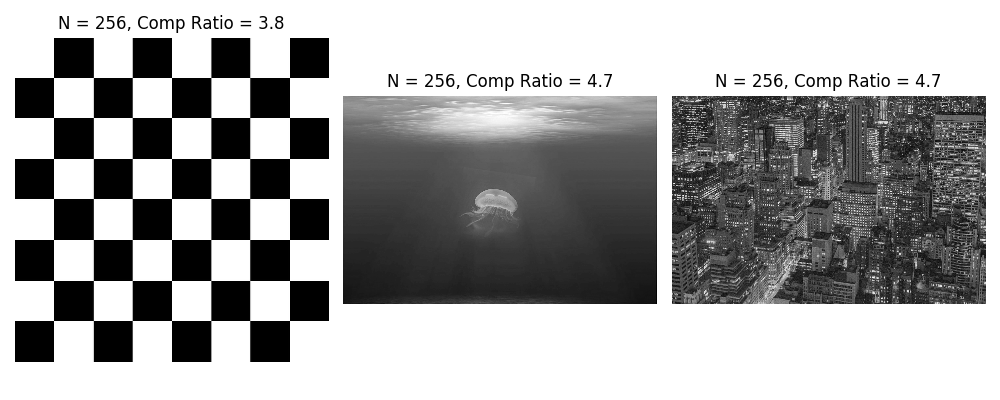
\includegraphics[width=1.0\linewidth]{../figs/img7.png}
    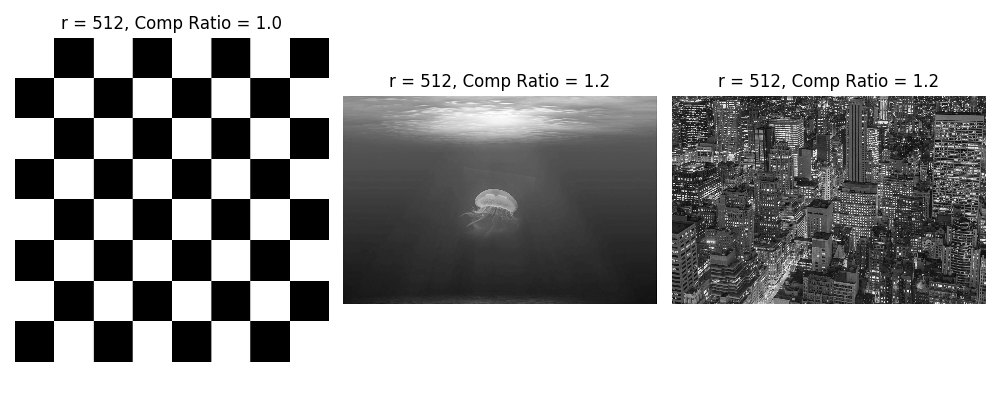
\includegraphics[width=1.0\linewidth]{../figs/img8.png}
\end{figure}


\section*{Appendix: Code}

\pagebreak

\lstinputlisting[language=Python, caption=oblig2.py, frame=full]{../src/oblig2.py}

\end{document}